%----------------------------------------------------------------------------------------
%	PACKAGES AND THEMES
%----------------------------------------------------------------------------------------
\documentclass[aspectratio=169,xcolor=dvipsnames]{beamer}
\usetheme{SimplePlusAIC}

\usepackage{hyperref}
\usepackage{csquotes}
\newcommand{\code}[1]{\texttt{#1}}
\usepackage{graphicx} % Allows including images
\usepackage{booktabs} % Allows the use of \toprule, \midrule and  \bottomrule in tables
\usepackage{svg} %allows using svg figures
\usepackage{tikz}
\usepackage{makecell}
\newcommand*{\defeq}{\stackrel{\text{def}}{=}}

%Select the Epilogue font (requires luaLatex or XeLaTex compilers)
\usepackage{fontspec}
\setsansfont{Epilogue}[
    Path=./epilogueFont/,
    Scale=0.9,
    Extension = .ttf,
    UprightFont=*-Regular,
    BoldFont=*-Bold,
    ItalicFont=*-Italic,
    BoldItalicFont=*-BoldItalic
    ]

%----------------------------------------------------------------------------------------
%	TITLE PAGE
%----------------------------------------------------------------------------------------

\title[Algebraic \& Geo. Comp. in OSCAR]{Algebraic and Geometric Computations in OSCAR} % The short title appears at the bottom of every slide, the full title is only on the title page
\subtitle{Author: Mara Belloti, Michael Joswig, Chiara Meroni, Victoria Schleis, and Johannes Schmitt}

\author[Ivan L. Ihwani]{Presented by: Ivan L. Ihwani}
\institute[SIAM NEWS SEPTEMBER 2023]{Department of Mathematics \newline National Central University}
% Your institution as it will appear on the bottom of every slide, maybe shorthand to save space


\date{September 21, 2023} % Date, can be changed to a custom date
%----------------------------------------------------------------------------------------
%	PRESENTATION SLIDES
%----------------------------------------------------------------------------------------

\begin{document}

\begin{frame}[plain]
    % Print the title page as the first slide
    \titlepage
\end{frame}

\begin{frame}{Overview}
    % Throughout your presentation, if you choose to use \section{} and \subsection{} commands, these will automatically be printed on this slide as an overview of your presentation
    \tableofcontents
\end{frame}

%------------------------------------------------
\section{Introduction to OSCAR}
%------------------------------------------------
\begin{frame}{Introduction to OSCAR}
\begin{figure}[h]

\includegraphics[width=4cm]{logos/OSCAR_logo.png}
\end{figure}
    \begin{itemize}
        \item \textcolor{blue}{\href{https://www.oscar-system.org/}{OSCAR}} (Open Source Computer Algebra Research) is a new open-source computer algebra system that is written in the \textcolor{blue}{Julia} programming language.
        \item Contributors: \textcolor{blue}{Wolfram Decker}, \textcolor{blue}{Claus Fleker}, \textcolor{blue}{Max Horn}, and \textcolor{blue}{Michael Joswig}. 
        \item Its ongoing development can be monitored on \href{https://github.com/oscar-system}{GitHub}.
        \item It is funded by the German Research Foundation within the collab. research center on \enquote{Symbolic Tools in Mathematics and Their Application.}
    \end{itemize}
\end{frame}

%------------------------------------------------
\begin{frame}{Introduction to OSCAR}
    \begin{itemize}
    \item It is easy to install OSCAR: on the Julia interactive command line, users can simply type:\\
        \code{import Pkg; Pkg.add("Oscar"); using Oscar}\\
        to download the relevant data from the internet and print a banner; \textcolor{blue}{OSCAR} is then ready for action!
        \item It works on every operating system (Linux, macOS, and Windows).
        \item OSCAR builds upon the collective capabilities of the \textcolor{red}{GAP} (group and representation theory), \textcolor{red}{Nemo/Hecke} (number theory), \textcolor{red}{polymake} (polyhedral and tropical geometry), and \textcolor{red}{Singular} (commutative algebra and algebraic geometry) packages. 
        %\item Its user interface draws inspiration from Donald Knuth's  \href{http://www.literateprogramming.com/knuthweb.pdf}{\textcolor{blue}{literate programming}} paradigm.
    \end{itemize}
\end{frame}


%-----------------------------------------------
\begin{frame}{OSCAR VS other software packages}
    \begin{itemize}
        \item Compared to \textcolor{blue}{\href{http://magma.maths.usyd.edu.au/magma/}{Magma}}, OSCAR is an accessible platform for interoperable and reproducible computations due to its open-source nature.
        \item Compared to \textcolor{blue}{\href{https://www.sagemath.org/}{SageMath}}, it is smaller but more tightly knit. Meaning: \textcolor{brown}{some computations that are possible in OSCAR are not currently achievable elsewhere}. Example: \textcolor{brown}{the computation of Galois groups of arbitrarily high degree}.
    \end{itemize}
\end{frame}

%------------------------------------------------
\section{Example: Parametric Volume of Polytope}

\begin{frame}{Parametric Volume of Polytope}
    \begin{itemize}
        \item \textcolor{blue}{In Convex Geometry Field $\Rightarrow$ Intersection Bodies (i.e. the Busemann-Petty Problem)}: this problem investigated whether a symmetric convex body with larger central \href{https://en.wikipedia.org/wiki/Hyperplane}{\textcolor{brown}{hyperplane}} sections must similarly have a larger volume. 
        \item The \href{https://github.com/micjoswig/oscar-notebooks/blob/master/SIAM-News/Parametrized_volume_of_slices.ipynb}{\textcolor{blue}{example}} presents an experimental approach to the problems by computing explicit instances of intersection bodies. 
        \item The methods exploit the fact that intersection bodies of polytopes are semi-algebraic — i.e., describable in terms of polynomial inequalities. 
        \item \textbf{The crucial step} is a parametric volume computation that requires methods from polyhedral geometry and commutative algebra, all of which exist in \textcolor{blue}{OSCAR}.
    \end{itemize}
\end{frame}

%--------------------------------------------------------------------------

\begin{frame}{Parametric Volume of Polytope}
    \begin{itemize}
        \item The algorithm in the notebook takes a polytope $P$
 as input; we are interested in slicing $P$ with arbitrary central hyperplanes.
 \item The slice volume function is a piecewise polynomial quotient, and the algorithm computes it explicitly.
 \item The method triangulates P, a standard step in polyhedral geometry, and then computes determinants of matrices with multivariate rational function entries, requiring basic linear algebra and efficient polynomial ring arithmetic.
 \item For conciseness, the \href{https://github.com/micjoswig/oscar-notebooks/blob/master/SIAM-News/Parametrized_volume_of_slices.ipynb}{\textcolor{blue}{example}} demonstrates the computation for one specific polytope: the truncated tetrahedron, an Archimedean solid (Figure 1).
    \end{itemize}
\end{frame}



%----------------------------------------------------------------------

\begin{frame}{Parametric Volume of Polytope}
    \begin{figure}[h]
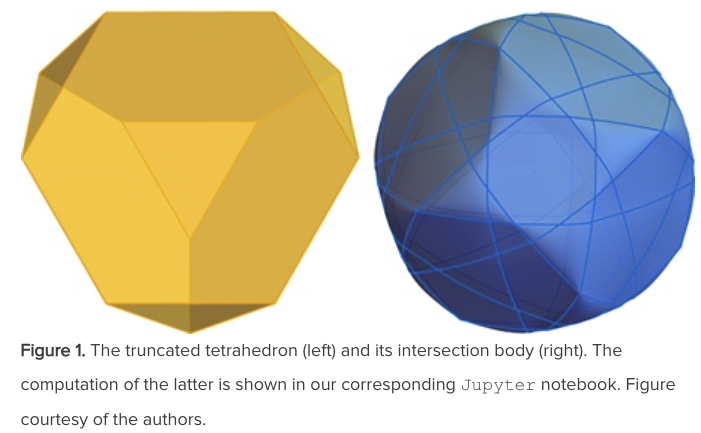
\includegraphics[width=10cm]{images/fig1.png}
\end{figure}
\end{frame}

%------------------------------------------------------------
%\begin{frame}{Parametric Volume of Polytope}
%    In this slide, some important text will be \alert{highlighted} because it's important. Please, don't abuse it.

%    \begin{block}{Block}
%        Sample text
%    \end{block}

%    \begin{alertblock}{Alertblock}
%        Sample text in red box
%    \end{alertblock}

%    \begin{examples}
%        Sample text in green box. The title of the block is ``Examples".
%    \end{examples}
%\end{frame}

%------------------------------------------------

%\begin{frame}{Multiple Columns}
 %   \begin{columns}[c] % The "c" option specifies centered vertical alignment while the "t" option is used for top vertical alignment

  %      \column{.45\textwidth} % Left column and width
   %     \textbf{Heading}
    %    \begin{enumerate}
     %       \item Statement
      %      \item Explanation
      %      \item Example
      %  \end{enumerate}

       % \column{.5\textwidth} % Right column and width
       % Lorem ipsum dolor sit amet, consectetur adipiscing elit. Integer lectus nisl, ultricies in feugiat rutrum, porttitor sit amet augue. Aliquam ut tortor mauris. Sed volutpat ante purus, quis accumsan dolor.

   % \end{columns}
%\end{frame}

%------------------------------------------------
\section{Other Examples}


%------------------------------------------------
\begin{frame}{Other Examples}
    \begin{itemize}
        \item \textcolor{brown}{\href{https://github.com/micjoswig/oscar-notebooks/blob/master/SIAM-News/Hurwitz_Combinatorics.ipynb}{Combinatorics of Hurwitz Numbers}}, tackle problems in enumerative algebraic geometry both in a combinatorial and algorithmic manner.
        \item \textcolor{brown}{\href{https://github.com/micjoswig/oscar-notebooks/blob/master/SIAM-News/Cox_rings_of_blow_ups_of_points.ipynb}{Cox Rings of Point Blow-ups}}, the problem in a geometry of varieties.
        \item \textcolor{brown}{\href{https://github.com/micjoswig/oscar-notebooks/blob/master/SIAM-News/Cox_rings_of_linear_quotients.ipynb}{Cox Rings of Linear Quotients}}, tackle a problem invariant theory field. 
        
    \end{itemize}
\end{frame}


\section{Installation}

\begin{frame}{Installation}
    \Huge{\centerline{\textbf{See The \href{https://www.oscar-system.org/}{Documentation}}}}
\end{frame}

%-----------------------------------------------------------
%\begin{frame}{Cox Rings of Linear Quotients}
 %   \begin{itemize}
  %      \item This \textcolor{blue}{\href{https://github.com/micjoswig/oscar-notebooks/blob/master/SIAM-News/Cox_rings_of_linear_quotients.ipynb}{example}} is related to the Cox ring of the \textcolor{blue}{Linear Quotient}. 
   %     \item Here, we must compute a certain \textcolor{blue}{invariant ring} and endow it with a nonstandard grading by a theorem of Ivan Arzhantsev and Sergey Gaĭfullin (mathematician in the Invariant Theory field). 
    %    \item Calculating this ring aids in examining the birational geometry of a linear quotient.
     %   \item \textbf{OSCAR} offers all the essential tools for efficiently handling matrix groups and their invariant theory.
    %\end{itemize}
%\end{frame}
%-------------------------------------------------------
%\begin{frame}{Table}
 %   \begin{table}
  %      \begin{tabular}{l l l}
   %         \toprule
    %        \textbf{Treatments} & \textbf{Response 1} & \textbf{Response 2} \\
     %       \midrule
      %      Treatment 1         & 0.0003262           & 0.562               \\
     %       Treatment 2         & 0.0015681           & 0.910               \\
     %       Treatment 3         & 0.0009271           & 0.296               \\
     %       \bottomrule
    %    \end{tabular}
    %    \caption{Table caption}
   % \end{table}
%\end{frame}

%------------------------------------------------

%\begin{frame}{Theorem}
 %   \begin{theorem}[Mass--energy equivalence]
 %       $E = mc^2$
 %   \end{theorem}
 %   \begin{equation}
 %       c^{2} = a^{2} + b^{2}
 %   \end{equation}
%\end{frame}

%------------------------------------------------

%\begin{frame}{Figure}
    %Uncomment the code on this slide to include your own image %from the same directory as the template .TeX file.
    %\begin{figure}
    %\includegraphics[width=0.8\linewidth]{test}
    %\end{figure}
%\end{frame}

%------------------------------------------------

%\begin{frame}[fragile] % Need to use the fragile option when verbatim is used in the slide
%    \frametitle{Citation}
 %   An example of the \verb|\cite| command to cite within the presentation:\\~

  %  This statement requires citation \cite{p1}.
%\end{frame}

%------------------------------------------------

\begin{frame}{References}
    % Beamer does not support BibTeX so references must be inserted manually as below
    \footnotesize{
        \begin{thebibliography}{99}
            \bibitem[Agostini A., Markwig, H., Noliau, C., Schleis, V., Sendra-Arranz, J., Sturmfels, B., 2022]{p1} Agostini A., Markwig, H., Noliau, C., Schleis, V., Sendra-Arranz, J., \& Sturmfels, B. (2022)
            \newblock Recovery of plane curves from branch points
            \newblock \emph{Preprint,} arXiv:2205.11287.
        \end{thebibliography}
        \begin{thebibliography}{99}
            \bibitem[Arzhantsev, I.V., \& Gaĭfullin, S.A., 2010]{p1} Arzhantsev, I.V., \& Gaĭfullin, S.A. (2010)
            \newblock Cox rings, semigroups and automorphisms of affine varieties
            \newblock \emph{Math. Sbornik,} 201(1), 3-24.
        \end{thebibliography}
        \begin{thebibliography}{99}
            \bibitem[Belotti, M., \& Panizzut, M., 2022]{p1} Belotti, M., \& Panizzut, M. (2022)
            \newblock Discrete geometry of Cox rings of blow-ups of $\mathbb{R}^3$
            \newblock \emph{Preprint,} arXiv:2208.05258.
        \end{thebibliography}
        \begin{thebibliography}{99}
            \bibitem[Berlow, K., Brandenburg, M.-C., Meroni, C., \& Shankar, I., 2022]{p1} Berlow, K., Brandenburg, M.-C., Meroni, C., \& Shankar, I. (2022)
            \newblock  Intersection bodies of polytopes
            \newblock \emph{Beitr. Algebra Geom.,} 63, 419-439.
        \end{thebibliography}
    }
\end{frame}

\begin{frame}{References}
    % Beamer does not support BibTeX so references must be inserted manually as below
    \footnotesize{
        \begin{thebibliography}{99}
            \bibitem[Breiding, P., \& Timme, S., 2018]{p1} Breiding, P., \& Timme, S. (2018)
            \newblock HomotopyContinuation.jl: A package for homotopy continuation in Julia
            \newblock \emph{Mathematical software – ICMS 2018,} pp. 458-465.
        \end{thebibliography}
        \begin{thebibliography}{99}
            \bibitem[Decker, W., Eder, C., Fieker, C., Horn, M., \& Joswig, M., 2024]{p1} Decker, W., Eder, C., Fieker, C., Horn, M., \& Joswig, M. (2024)
            \newblock The OSCAR book
            \newblock \emph{To be published} .
        \end{thebibliography}
        \begin{thebibliography}{99}
            \bibitem[Fieker, C., Hofmann, T., \& Joswig, M., 2022]{p1} Fieker, C., Hofmann, T., \& Joswig, M. (2022)
            \newblock Computing Galois groups of Ehrhart polynomials in OSCAR
            \newblock \emph{Sém. Lothar. Combin.,} 86B, 87.
        \end{thebibliography}
        \begin{thebibliography}{99}
            \bibitem[ Gardner, R.J., Koldobsky, A., \& Schlumprecht, T., 2022]{p1}  Gardner, R.J., Koldobsky, A., \& Schlumprecht, T. (2022)
            \newblock An analytic solution to the Busemann-Petty problem on sections of convex bodies
            \newblock \emph{Ann. Math.,} 149(2), 691-703.
        \end{thebibliography}
    }
\end{frame}

\begin{frame}{References}
    % Beamer does not support BibTeX so references must be inserted manually as below
    \footnotesize{
        \begin{thebibliography}{99}
            \bibitem[ Klartag, B., \& Milman, V., 2022]{p1}  Klartag, B., \& Milman, V. (2022)
            \newblock The slicing problem by Bourgain.  In A. Avila, M.T. Rassias, \& Y. Sinai (Eds.)
            \newblock \emph{Analysis at large: Dedicated to the life and work of Jean Bourgain,} (pp. 203-231). Cham, Switzerland: Springer Cham.
        \end{thebibliography}
        \begin{thebibliography}{99}
            \bibitem[Knuth, D.E., 1984]{p1} Knuth, D.E. (1984)
            \newblock  Literate programming
            \newblock \emph{Comp. J.,} 27(2), 97-111.
        \end{thebibliography}
}
\end{frame}

%------------------------------------------------

\begin{frame}
    \Huge{\centerline{\textbf{Thank You}}}
\end{frame}

%----------------------------------------------------------------------------------------
\end{document}